\documentclass{article}

% if you need to pass options to natbib, use, e.g.:
% \PassOptionsToPackage{numbers, compress}{natbib}
% before loading nips_2018

% ready for submission
% \usepackage[final]{nips_2018}

% to compile a preprint version, e.g., for submission to arXiv, add
% add the [preprint] option:
% \usepackage[preprint]{nips_2018}

% to compile a camera-ready version, add the [final] option, e.g.:
% \usepackage[final]{nips_2018}

% to avoid loading the natbib package, add option nonatbib:
\usepackage[nonatbib, final]{nips_2018}

\usepackage[utf8]{inputenc} % allow utf-8 input
\usepackage[T1]{fontenc}    % use 8-bit T1 fonts
\usepackage{hyperref}       % hyperlinks
\usepackage{url}            % simple URL typesetting
\usepackage{booktabs}       % professional-quality tables
\usepackage{amsfonts}       % blackboard math symbols
\usepackage{nicefrac}       % compact symbols for 1/2, etc.
\usepackage{microtype}      % microtypography

\usepackage[backend=biber,sorting=none]{biblatex}
\addbibresource{references.bib}
\usepackage{float}
\usepackage{graphicx}
\graphicspath{{images/}}

\usepackage[most]{tcolorbox}
\newtcolorbox{mybox}[2][]{%
  attach boxed title to top center
               = {yshift=-8pt},
  colback      = black!5!white,
  colframe     = black!75!black,
  fonttitle    = \bfseries,
  colbacktitle = black!85!black,
  title        = #2,#1,
  enhanced,
}  % source: https://latex.org/forum/viewtopic.php?t=29038


\usepackage{fancyhdr}
\pagestyle{fancy}

\title{Population Based Training of Neural Networks:\\ a comparison against Grid Search}

% The \author macro works with any number of authors. There are two
% commands used to separate the names and addresses of multiple
% authors: \And and \AND.
%
% Using \And between authors leaves it to LaTeX to determine where to
% break the lines. Using \AND forces a line break at that point. So,
% if LaTeX puts 3 of 4 authors names on the first line, and the last
% on the second line, try using \AND instead of \And before the third
% author name.

\author{
  Fernando Díaz\hspace{2em} Giorgio Ruffa\\\\
  \texttt{\{fdiaz, ruffa\}@kth.se} \\
  %% examples of more authors
  %% \AND
  %% Affiliation \\
  %% Address \\
  %% \texttt{email} \\
  %% \AND
  %% Coauthor \\
  %% Affiliation \\
  %% Address \\
  %% \texttt{email} \\
  %% \And
  %% Coauthor \\
  %% Affiliation \\
  %% Address \\
  %% \texttt{email} \\
  %% \And
  %% Coauthor \\
  %% Affiliation \\
  %% Address \\
  %% \texttt{email} \\
}

\renewcommand{\headrulewidth}{0pt}
\lhead{II2202, Fall 2018, Period 1-2}
%% or \lhead{II2202, Fall 2016, Period 1}
\chead{Final Report}
\rhead{\today}

\providecommand{\keywords}[1]{\textbf{\textit{Keywords:}} #1}


\begin{document}
% \nipsfinalcopy is no longer used

\maketitle
\thispagestyle{fancy}

\begin{abstract}
The training and performance of modern neural networks largely depend on the choice of hyperparameters, which is usually empirically driven. Population Based Training is a recently introduced method to automatically perform hyperparameters tuning that promises to use less computational resources while achieving comparable or better results than more traditional methods. Given the novelty of the approach, little is known about the real trade-off between accuracy and computational resources used.
Trough a rigorous and fair comparison of population based training against grid search, by means of controlled simulations on well established data sets, our qualitative results confirms that the former consistently outperforms the latter and, in some conditions, only using one sixth of the computational resources, thus fostering the need of a further quantitative investigation.

\end{abstract}

\keywords{Deep Learning, Neural Networks, Optimization Methods, Tuning}


\tableofcontents


\section*{List of Acronyms and Abbreviations}
\label{list-of-acronyms-and-abbreviations}
\begin{itemize}
    \item \textbf{PBT} Population Based Training
    \item \textbf{CNN} Convolutional Neural Network
    \item \textbf{MLP} Multi-layer Perceptron
    \item \textbf{FCN} Fully Connected Network
    \item \textbf{GS} Grid Search
    \item \textbf{DL} Deep Learning
    \item \textbf{AI} Artificial Intelligence
\end{itemize}



\section{Introduction}
	\label{sect:introduction}
	
	At the heart of the machine learning approach, there is, indeed, the act of learning the parameters that define the model. This operation is itself governed by a set of variables, the so-called ``hyperparameters'', which can vary in number and complexity, depending on the model being trained and on the optimization algorithm used.
	
	Unlike parameters, hyperparameters are usually set by hand by the practitioner, and they can hugely impact the time required to train the model, as well as it's predictive capabilities. A rather simple example is the effect on the training error of the learning rate $\alpha$, which is used in all the families of gradient descent algorithms. If alpha is too large, the training error may increase rather than decrease; if it is too small, the training will be sensibly slower and the error may be even settle on a high value\footnote{Compared to the error obtained with a lower $\alpha$.} (pp. 424 of \cite{Goodfellow-et-al-2016}).
	
	Despite the clear importance of hyperparameters, there is little agreement on their correct initialization and how should they be chosen depending on the problem being modeled. Scientists often use a wide set of rules-of-thumb and, more importantly, their experience to achieve better results; In fact, whole books have been dedicated to the collection of this knowledge\cite{DBLP:series/lncs/7700}.
	
	The common approach to mitigate this empiricism is the use of automated algorithms for hyperparameters tuning. This field has recently seen the rise in popularity of sophisticated methods that borrow ideas and concepts from evolutionary computing in order to speed-up the convergence by finding better hyperparameters (please see section \ref{sec:th_framework} for further details).
	Precisely in this framework, is quite recent the introduction of a new method called Population Based Training\cite{PBT} (from now on \emph{PBT}) to perform automatic optimization of neural networks hyperparameters.
	
	Although PBT has been introduced in multiple popular libraries for hyperparameter tuning\cite{Kim2018CHOPTA}\cite{Liang2018RayR}, and experiments regarding its performance have been performed in various deep learning areas\cite{PBT}, there is still, to the best of our knowledge, a lack of information on how it performs on simpler architectures like Multi-layer Perceptrons (MLP) and Convolutional Neural Networks (CNN), especially against more established practices like grid search. The use of similar approaches obtained promising results while training convolutional neural networks \cite{pmlr-v70-real17a}, but at a very high computational cost, which PBT promises to minimize.
	
	This study aims to investigate how PBT behaves while employed on simpler models like MLP and CNNs; in particular, how it compares with grid search while taking into account the computational resources used.
	
	\subsection{Theoretical Framework}
	\label{sec:th_framework}
	In this section, we review the salient theory concerning hyperparameters optimization in the deep learning area by reviewing the methods commonly used and the new state of the art techniques. We will also present how PBT takes inspiration from all these methods while still maintaining a rather simple mechanic.
	
	\subsubsection*{Manual Tuning}
	For its very own nature, manual tuning is the most empiric approach, as it is totally based on the proficiency of the practitioner and his knowledge of the learning algorithm used. It usually implies a trial-and-error approach, where a series of sequential runs are performed, usually once at a time, varying one or more hyperparameter values. A set of guidelines can be followed building upon knowledge gathered by other practitioners \cite{Goodfellow-et-al-2016}\cite{DBLP:series/lncs/7700}\cite{LeCun:1998:EB:645754.668382}.
	The methods offer little guarantees of reproducibility; moreover, hyperparameters obtained for training the final model are seldom reported in the literature. 
	It has, although, a significant upside. The practitioner can interrupt the training as soon as the results of the change do not seem to be promising, thus saving computational power and time. Needless to say, this technique requires full human supervision, thus limiting the amount of exploitable parallelization. 
	
	\subsubsection*{Grid Search}
	For each hyperparameter, the user selects a small finite set of values to explore. The grid search algorithm then trains a model for every joint specification of hyperparameter values in the Cartesian product of the set of values for each individual hyperparameter. The experiment that yields the best validation set error is then chosen as having found the best hyperparameters.
	It is the most straightforward automatic algorithm for hyperparameter tuning and is considered to perform well when a low number of hyperparameters is explored\cite{Bergstra:2012:RSH:2188385.2188395}. The clear downside is that the computational cost grows exponentially as the number of hyperparameters grows.
	Despite this aspect, it has been used successfully to train various deep learning models \cite{Larochelle:2007:EED:1273496.1273556}\cite{He2016DeepRL}.
	
	\subsubsection*{Random Search}
	In random search, a marginal distribution is defined for each hyperparameter, which is then sampled to obtain a series of unique independent combinations of hyperparameters. It is considered to converge faster than grid search when a high number of hyperparameters is explored\cite{Bergstra:2012:RSH:2188385.2188395}, especially when several of them do not have a significant impact on the validation error. Compared to grid search, where runs on the same dimension share the same, potentially unfruitful, hyperparameter, random search can explore the search space more efficiently.
	
	\subsubsection*{Sequential Optimization}
	In sequential optimization, fewer optimization processes (compared with random or grid search) are used with an initial tentative set of hyperparameter. As the training progresses, depending on the outcome of the previous generation of optimization processes, a new, hopefully, better performing, set of hyperparameter is used. The intuition behind this method is to mimic the process of a human practitioner, that incrementally refines the set of hyperparameters depending on the training behavior.
	Important techniques developed in this field are  Gaussian Process (GP) and Tree-structured Parzen Estimator (TPE)\cite{Bergstra:2011:AHO:2986459.2986743}.
	
	\subsubsection*{Evolutionary Approaches}
	Very recently the field of evolutionary computing has seen the introduction of machine learning techniques, obtaining interesting and promising results \cite{Zhang:2011:ECM:2772968.2773017}\cite{XueZhang2016}. The approach was also extended in the opposite direction: using evolutionary techniques to scan more efficiently the hyperparameter space of machine learning models\cite{pmlr-v70-real17a}. In this kind of framework, each learning task is considered as an individual of a population. Periodically the performance of each individual is assessed, and the most performing ones are crossed and then mutated. The key aspect of these techniques is that they abort the search in unpromising parts of the search space before the full training process is completed, in order to reallocate the computational resources in the regions of the search space that seem more promising, thus to mimic the behavior of a human practitioner further.
	\textit{Real et al.}\cite{pmlr-v70-real17a} developed a fully evolutionary approach to create complete CCN architectures that were able to obtain results comparable to the state of the art, but \textit{``despite significant computational requirements''} were used (see section \ref{sec:literatureStudy} for further details). 
	
	\subsubsection*{Knowledge Transfer}
	Knowledge transfer is not an algorithm for automatic hyperparameters tuning, but a recent technique in which the information contained in a model can be transferred to another model without involving a retraining phase, thus saving consistent computational power otherwise used to re-train the second model \cite{Chen2015Net2NetAL}\cite{Wei:2016:NM:3045390.3045451}.
	
	
    \subsubsection*{PBT as a Pragmatic Synthesis}
    Borrowing mainly from the evolutionary approaches reported above, PBT involves a set of independent learners called \textit{``individuals''} which pertains to a \textit{``population''} that are trained in parallel with a random set of hyperparameters\footnote{An aspect very similar to random search.}\footnote{Although for this work, as we will explain later in section \ref{sec:method}, we are going to modify how the members of the population are initialized.}. This independent training phase is called a \textit{``step''}, which has a fixed duration expressed in the number of epochs, that is usually only a fraction of the total number of epochs necessary to reach convergence. On \textit{step} completion, the individuals are ranked depending on their performance on the validation set\footnote{The loss or the accuracy can be used}. Underperforming individuals are then replaced by better-performing ones. This is done by copying their hyperparameters and parameters on the now free individuals. This phase is called \textit{``exploitation''} and, at a very basic level, is an instance of knowledge transfer.
    The final phase is called \textit{``perturbation''} and consists of randomly perturbing the hyperparameters of the copied individuals in the proximity of the promising ones. The \textit{perturbation} phase strictly resembles the random search approach, in which no pair of learners share a single hyperparameter value. At this point, the ``step'' phase starts again, and all the phases are repeated until a \textit{``good enough''} solution is found, exactly as a human practitioner would do (see figure \ref{fig:PBTStep}).
    
    \begin{figure}[H]
        \label{fig:PBTStep}
        \centering
        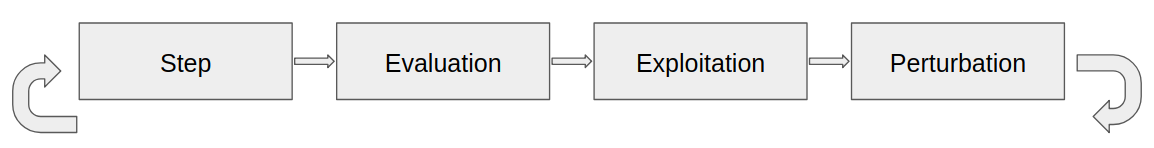
\includegraphics[width=\textwidth,height=\textheight,keepaspectratio]{PBT_step}
        \caption{PBT execution flow chart.}
    \end{figure}
    
    The significant difference between PBT and the approach reported in \cite{pmlr-v70-real17a}, is that PBT does not aim to identify a whole network architecture, but is instead focused only on the hyperparameters that influence the training phase (i.e. learning rate, dropout probability, l1 and l2 regularization, etc.). Thus reducing sensibly the computational effort necessary to perform the tuning and simultaneously simplifying the complexity of the algorithm.
    
    PBT has obtained promising results on the following deep learning areas: deep reinforcement learning, supervised learning for machine translation, generative adversarial networks \cite{PBT}.
    Moreover, the authors claim the method has “[...] a wall-clock run time that is no greater than that of a single optimization process, does not require sequential runs and is also able to use fewer computational resources than naive search methods such as random or grid search"\cite{PBT}. 
    
    Regarding their claim of lack of sequential runs, we must say that while the step phase is completely parallelizable (as all the individuals are independent), the evaluation exploitation and perturbation phase must be performed synchronously.


\subsection{Literature Study}
\label{sec:literatureStudy}

The book by \textit{Goodfellow et al} \cite{Goodfellow-et-al-2016} offers a good review of the importance and nature of hyperparameters tuning for deep learning, we suggest the reading of chapter 11. 

The book by \textit{Geron Aurelien}\cite{Gron:2017:HML:3153997} treats the issue from a more practical stance; the first two chapters are of most interest.

The curated collection by \textit{Montavon et al}\cite{DBLP:series/lncs/7700} contains a set of salient papers concerning best practices and "\textit{tricks}" for hyperparameters selection and tuning for deep learning applications. The introduction clearly points out the empirical nature of the task of hyperparameters optimization and how the necessity of a corpus of best practices outgrows from the popularity of dedicated workshops of the famous NIPS conference. The collection contains the popular paper \textit{Efficient Backprop} by \textit{LeCun et al}\cite{LeCun:1998:EB:645754.668382} which entails the effects of an improper value of the learning rate (and much more), as reported above.

\textit{Larochelle et al} \cite{Larochelle:2007:EED:1273496.1273556}, performed a wide set of experiments in which grid search was extensively used to perform hyperparameters tuning. The aim was to show the promising capabilities of deep learning systems in solving problems with many factors of variation.

\textit{Bergstra and Bengio} \cite{Bergstra:2012:RSH:2188385.2188395}, demonstrates the validity of random-search as a more effective mean of hyperparameters tuning compared to grid search. Section 2.1 describes a formal procedure to estimate test set accuracy while taking into account any uncertainty in the choice of which trial is actually the best-performing one\footnote{Unfortunately the test involves an extensive use of computational resources which are not at our disposal.}. It also shows that grid search is more reliable in low dimensional spaces\footnote{This is one of the reasons we opted for grid search rather than random-search, as our computational resources forced us to work with a low number of hyperparameters to tune}.

\textit{Bergstra et al} \cite{Bergstra:2011:AHO:2986459.2986743}, shows that random search is unreliable for the training of deep belief networks, while sequential algorithms find significantly better results.

The survey by \textit{Zhang et al} \cite{Zhang:2011:ECM:2772968.2773017}, outlines a clear taxonomy for classifying the employment of machine learning techniques (including artificial neural networks) in the realm of evolutionary computation. The importance of the usage of the two approaches in conjunction is clearly stated and signals the need for a better understanding of a trade-off between the computation burden introduced by the machine learning approach and its advantages.

\textit{Real et al}\cite{pmlr-v70-real17a} apply a fully genetic approach with a complex set of mutation operators. Their method is focused on the generation of a fully trained convolutional architecture rather than the tuning of hyperparameters (the learning rate constitutes an exception). They also perform the copy of the weights between parent and child individuals. \textit{``Despite significant computational requirements''}\cite{pmlr-v70-real17a}, they show that it is possible to reliably evolve models with performances comparable to the state of the art for the CIFAR10\cite{CIFAR10} and CIFAR100\cite{CIFAR100} data-sets, without any human intervention after the beginning of the procedure.

\textit{Chen, Goodfellow and Shlens}\cite{Chen2015Net2NetAL}, develop a method of knowledge transfer between an already trained network and its evolution, thus greatly improving the training time. They demonstrate that their approach is able to obtain state of the art accuracy rating on the ImageNet data-set by increasing depth on Inception modules.

\section{Problem and Knowledge Gap}
As stated in the introduction, the final performance of a deep learning model may depend strongly on the experience and proficiency of the practitioner, thus resulting in a very empirical approach \cite{Goodfellow-et-al-2016}\cite{DBLP:series/lncs/7700}.
One of the consequences of this situation is that the computational budget dedicated to the development of a learning algorithm has seen an important shift from the CPU cycles used to evaluate the hyperparameter choice (i.e. by tuning the regular parameters), to the ones spent for hyperparameter exploration. A situation particularly significant in the field of image classification \cite{10.1371/journal.pcbi.1000579}\cite{Coates:2011:IEV:3104482.3104598}.

Another direct consequence of the aforementioned empiric approach is that it directly implies a lack of reproducibility, which poses an obstacle to scientific advancement\cite{Bergstra:2011:AHO:2986459.2986743}.

Algorithmic approaches to hyper-parameter optimization are seen as a solution. By the words of Bergstra et al., \textit{``[They] make machine learning
results easier to disseminate, reproduce, and transfer to other domains. [...] Powerful hyper-parameter optimization algorithms broaden the horizon of
models that can realistically be studied; researchers need not restrict themselves to systems of a few variables that can readily be tuned by hand.''}\cite{Bergstra:2011:AHO:2986459.2986743}
These words underline the importance of efficient hyperparameter tuning on the computational intensive areas of machine learning (deep learning above all). 

Given the promising results obtained by PBT\cite{PBT} in various DL areas (reinforcement learning, machine translation and generative adversarial networks) while compared with grid search and of similar evolutionary approaches\cite{pmlr-v70-real17a}, we aim to investigate if PBT can achieve comparable results in the field of MLP and CNN training. Despite being areas that require extensive computational resources, there are no records, to the best of our knowledge, of PBT performance in these fields of deep learning.

\subsection{Research Question}
\label{sect:questions}
Efficient and automatic optimization is central to the development of DL models.
PBT has recorded to obtain a comparable or better accuracy than grid search in many deep learning areas\cite{PBT}.

\begin{mybox}[colback = white, width = \textwidth]{Research Question}
Can PBT obtain a comparable or better accuracy than grid search while training Multi-layer Perceptrons and Convolutional Neural Networks? 
    
If yes, can it do it with less computational resources?
\end{mybox}
\begin{mybox}[colback = white, width = \textwidth]{Hypothesis}
Due to the promising results reported in the literature, we think PBT can achieve better results with significantly less computational resources employed.
\end{mybox}


\section{Method}
\label{sec:method}
We aim to obtain a comparison of the accuracy obtained by PBT and grid search with the following architectures: Multi-Layer Perceptron and LeNet-5\cite{LeNet5}.

The former is trained on the Boston Housing data-set\cite{harrub78}, which is a regression problem. While the latter on the well-renowned MNIST data-set\cite{lecun-mnisthandwrittendigit-2010}, a classic image classification problem.

The method chosen to answer the research question is the empirical method, as several aspects justify this decision. First of all, the dynamics of the training phase of a neural network are mostly unknown, especially the effect of hyperparameters. Analytic methods are seldom, if not never, used\footnote{The existence of a complete analytic model would render useless all the effort in developing a good automatic algorithm for hyperparameter tuning.}. Moreover, it is an established practice in the literature to always back any claim with experimental results\cite{pmlr-v70-real17a}\cite{Bergstra:2012:RSH:2188385.2188395}\cite{Larochelle:2007:EED:1273496.1273556}\cite{Bergstra:2011:AHO:2986459.2986743}. However, the resources at our disposal are clearly not sufficient to perform an extensive quantitative analysis at the level of the ones reported in the literature. For this reason, the scope of this work is limited to a qualitative analysis were a very limited set of simulation can be performed\footnote{In works like \cite{pmlr-v70-real17a}, \cite{Bergstra:2012:RSH:2188385.2188395} and \cite{Bergstra:2011:AHO:2986459.2986743}, thousands of simulations are performed on dedicated GPU clusters.}. For further details please see section \ref{sec:discussion}. 

The work was divided into three phases: setup, data collection, analysis.
The setup includes the installation of the TensorFlow software package and the implementation of the PBT algorithm along with the tools necessary to collect metrics on the actual performances of the method.
In the data collection phase, we performed the PBT method and the grid search method first on the MLP architecture and then on the image classification problem. This decision gave us the possibility to iterate quickly in case the tools developed needed to be modified, as the wall-time necessary to train an MLP model is just a fraction of the one needed by a CNN. The main metrics that was recorded is the value of the loss function on the validation set. Note that the expression of the loss function varies depending on the kind of problem being modeled (see section \ref{sec:results} for further details).
Finally, the collected data were analyzed and the results are reported in section \ref{sec:results}.

The question that arises now is how to compare the two approaches, PBT and grid search, in a fair way. There are a series of factors that have to be controlled. 

First of all, there is the node of how to measure the computational resources implied. It will be very difficult to link it to hardware specifications, hence, for this reason, we are going to follow a more abstract approach. We will consider the number of “workers” used, that is, the number of maximum independent models that can be trained simultaneously, which, in turns, corresponds to a unique set of hyperparameters that can be used at the same time. To better clarify, in the case of grid search this number coincides with the total number of possible combination of hyperparameters (i.e 2 hyperparameters with 6 possible values is a $6 \times 6 = 36$ nodes grid); in case of PBT, it coincides with the number of individuals in the population. The careful reader will have noticed that time (either wall time or CPU time) is not a considered factor; hence we are totally focused on the computational resources employed as the independent variable and the loss function of the validation set as the dependent variable.

Secondly, we need to control any contribution given by randomization (i.e. dropout and/or initialization of weights), at least ensuring that the distributions used are the same in each worker. 

Thirdly, we need to have full control of the dataset and how the training, testing and validation sets are generated, ensuring they are the same both for grid search and PBT.

The aforementioned factors influenced how the implementation phase is performed. For a given and well-defined network architecture, we fix the initialization method, hence all the workers share the same one. Then the number of hyperparameters to tune and the granularity of the grid is selected. Given our limited resources we preferred to limit our investigation to a bi-dimensional hyperparameter grid.

The grid search is performed first, using the full grid, and the best performing worker is taken as the baseline (i.e. the result that PBT has to beat). Then, keeping the same training and validation set, PBT is executed on the same number of epochs used for grid search, using a population of the same size as the nodes in the grid. This step is aimed to verify if, with the same computational resources, PBT can obtain a comparable or better result than grid search. Note that PBT individuals are always initialized with the same hyperparameters as the grid search workers, hence having the exact same starting point. To evaluate what is the performance of PBT when fewer resources are employed, we decrease gradually the number of individuals in the population\footnote{Note that the number of individuals is constant for the whole training. That is until the same number of epochs used to train grid search are passed.}. The individuals will still share the same starting hyperparameters used by grid search, but given their lower number, a sub-sampling will be performed (see figure \ref{fig:subsampling}).

\begin{figure}[H]
    \label{fig:subsampling}
    \centering
    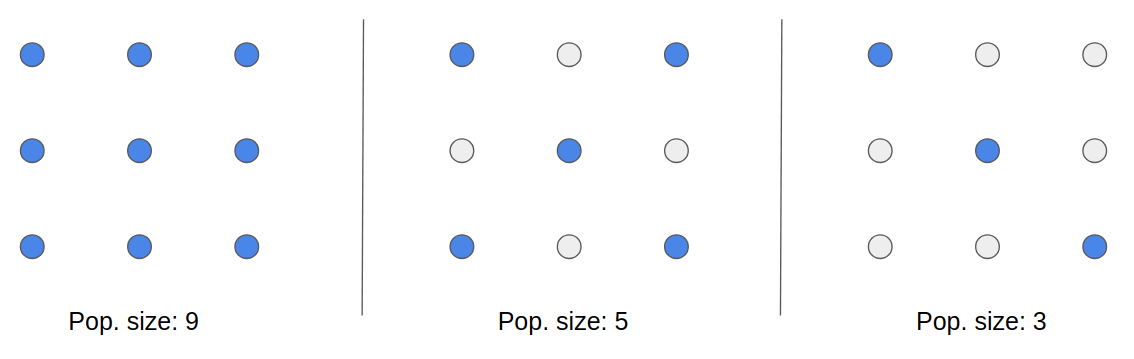
\includegraphics[width=\textwidth,height=\textheight,keepaspectratio]{subsampling}
    \caption{Progressive sub-sampling of the hyperparameters grid}
\end{figure}

The best performing PBT individual of each population is taken as the optimal result and the value of his loss function is compared with the grid search baseline.

\section{Results and analysis}
\label{sec:results}

This section contains the results obtained following the method reported in section \ref{sec:method}.

\subsection{Multi-Layer Perceptron}
\label{sec:fcnn}

In this section, we train a neural network to predict the price of a house in the Boston area, given information such as the average number of rooms per dwelling, areas of non-retail business in the town, the age of people who own the house, and many other attributes. During training, we aim to reduce the root mean squared error (RMSE) between the predicted value and the actual house price.

The architecture of the neural network used is quite simple, with just one hidden layer with 64 neurons and ReLU activation functions. Although for this problem the model is not very sensitive to the choice of hyperparameters, our goal is to show that even in this kind of scenarios, PBT can find a better set of hyperparameters than GS, while also reducing the generalization error.

We will perform two experiments: in the first one, the starting grid of hyperparameters is far away from the optimal hyperparameters. In the second one, we center the grid around the best hyperparameters.

Regarding PBT, we use population sizes between 6 and 36, where each member contains a set of hyperparameters sampled from the grid as it was explained in Sec. \ref{sec:method}. We use the following configuration to train the population:

\textbf{Hyperparameters}: we only allow to change two hyperparameters.

\textbf{Step}: each iteration does a step of gradient descent on a batch of data (32) using the Adam optimizer.

\textbf{Eval}: we evaluate a model computing the RMSE loss on the validation set.

\textbf{Ready}: a member is deemed ready to enter the exploit-explore phase every 50 iterations.

\textbf{Exploit}: we rank all the members in the population by their loss in the evaluation set (ascending). If a member $M^-$ is in the bottom 20\% of the rank, we sample a member $M^*$ uniformly from the top 20\%, and we copy the value for the hyperparameters of $M^*$ to $M^-$.

\textbf{Explore}: we randomly perturb the hyperparameters by a factor of 0.2, 0.5, 1.5 or 2.

\subsubsection{Bad grid choice}

In this example, we try to apply strong regularization to a problem that, from our experience, does not need too much regularization. We use a grid search with 36 combinations of hyperparameters to build our baseline. To construct the grid, we get 6 values evenly spaced on a log scale from 0.1 to 0.2. These values will be assigned to the range of possible values for l1 and l2 regularization.

\begin{verbatim}
l1_values = [0.01, 0.01825, 0.0331, 0.06034176336545162, 0.1099, 0.2]
l2_values = [0.01, 0.01825, 0.0331, 0.06034176336545162, 0.1099, 0.2]
\end{verbatim}

Hence, it is evident that the combination of hyperparameters would be as follows:
$$
Grid = \{C_1 = (0.01, 0.01), C_2 = (0.01, 0.01825), \cdots, C_{35} = (0.2, 0.1099), C_{36} = (0.2, 0.2)\}
$$

\subsubsection*{Results}

The best Grid Search model have a loss of \textbf{27.87} (l1 = \textit{1e-2} and l1 = \textit{1e-2}) on the validation set. We will refer to this result as \textit{baseline}.

To beat this score, we trained populations of different sizes using the PBT algorithm. Among all the populations, the best member have a loss of \textbf{22.1} (l1 = \textit{1e-5} and l2 = \textit{1e-5}). This member belongs to the population of size 30. We can already see that the best value for the hyperparameters of this member are far away from the limits of the grid that we used to initialize the population.

Moreover, as it is shown in Fig. \ref{fig:training-curves}, all the population members beat the baseline. Although the difference of some populations with the baseline might seem marginal, we must take into account that, for example, a population of size 18 takes less computational resources to train (ideally half) than to execute a grid search with 36 models.

\begin{figure}[H]
    \label{fig:training-curves}
    \centering
    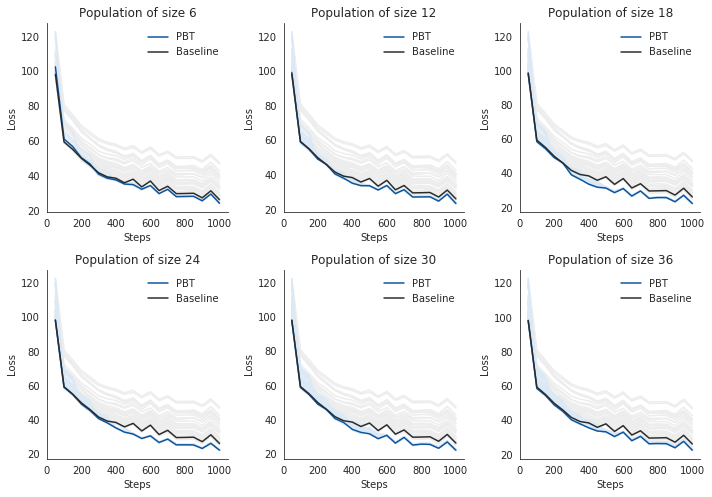
\includegraphics[width=\textwidth,height=\textheight,keepaspectratio]{training_curves}
    \caption{Training curves for Grid Search and PBT. Each worker is represented by a line. Highlighted lines are an average of the top 5 models at each step}
\end{figure}

As we can see, as we increase the size of the population, the performance gap between the top workers of each approach also widens.

In Fig. \ref{fig:hyp}, we can see the different values that the
hyperparameters take during PBT for a population of size 36.

\begin{figure}[H]
    \label{fig:hyp}
    \centering
    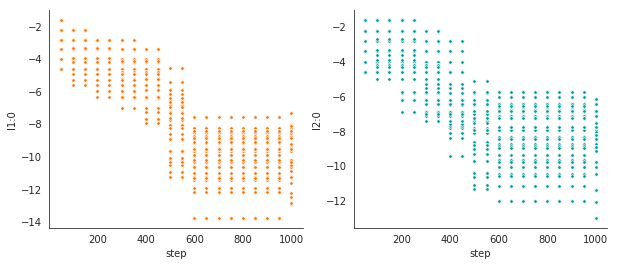
\includegraphics[width=\textwidth,height=\textheight,keepaspectratio]{hyperparameter_population.png}
    \caption{l1 (left) and l2 (right) regularization values (in a log scale). Each marker represents the value for the corresponding hyperparameter of one worker at a specific step}
\end{figure}

Finally, in Fig. \ref{fig:evol} we show a visual comparison between the hyperparameter values explored during PBT and the values in the grid.

\begin{figure}[H]
    \label{fig:evol}
    \centering
    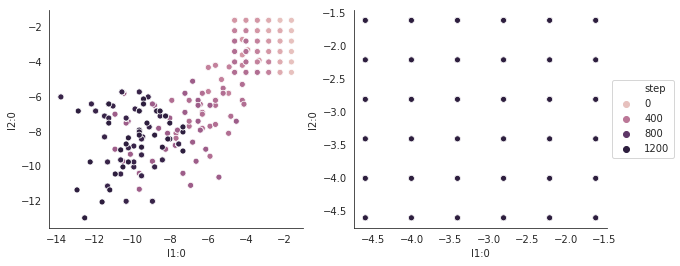
\includegraphics[width=\textwidth,height=\textheight,keepaspectratio]{hyperparameter_evolution.png}
    \caption{l1 (x-axis, log scale) and l2 (y-axis, log scale) regularization values explored during PBT (left), and grid search (right). As it is obvious, during grid search, values don't change. A darker color represents a value explored in a later stage (step) during training.}
\end{figure}

\subsubsection{Good grid choice}
\label{sec:goodgrid}

Taking a look at Fig. \ref{fig:evol}, one can argue that, since the best hyperparameters reside outside the grid, it is easier for PBT to beat grid search given that the baseline we built using the last method is not very strong. For this reason, in the following experiment, we are going to center the intervals used to build the grid around the best hyperparameters.

For this second experiment we will allow to tune l1 and the dropout rate (introduced after the hidden layer), using the following starting grid:

\begin{verbatim}
l1_values = [0.0001, 0.000458, 0.002091, 0.0095643, 0.043734, 0.2]
dr_values = [0.01, 0.0182, 0.0331, 0.0603, 0.10985605433061178, 0.2]
\end{verbatim}

As you can see, the best l1 values found during the last experiment are around the center of the \texttt{l1\_values} interval.

We obtained the following learning curves:

\begin{figure}[H]
    \label{fig:training-curves2}
    \centering
    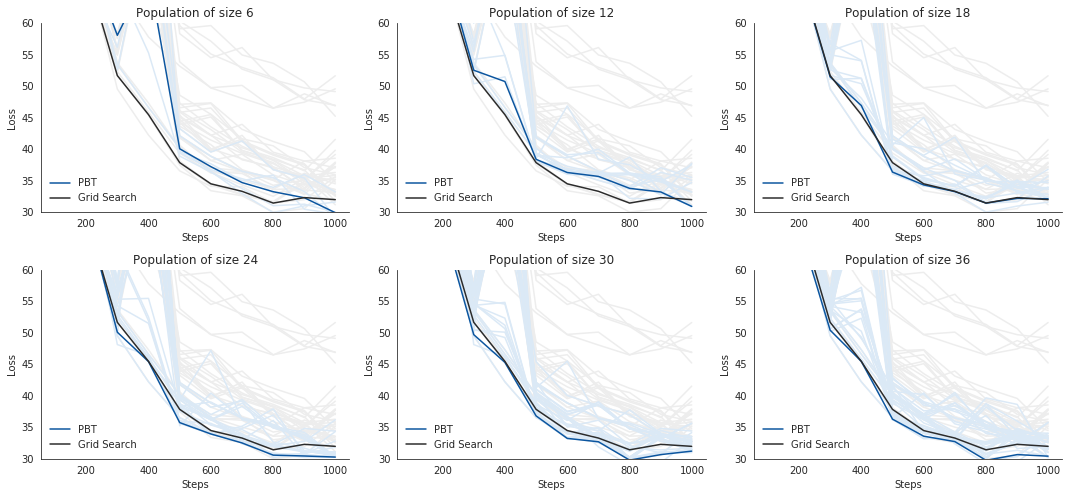
\includegraphics[width=\textwidth,height=\textheight,keepaspectratio]{training_curves2}
    \caption{Training curves for Grid Search and PBT. Each worker is represented by a line. Highlighted lines are an average of the top 5 models at each step}
\end{figure}

As expected, the difference between PBT and Grid Search now is marginal, but still, most PBT populations beat the baseline, even those with a number of members lower than the number of cells in the grid (36).

The evolution of the hyperparameters (Fig. \ref{fig:hyp2}) is slightly different. Now the l1 regularization values (left) do not take the lowest possible values. On the contrary, the dropout rate values do (right).

\begin{figure}[H]
    \label{fig:hyp2}
    \centering
    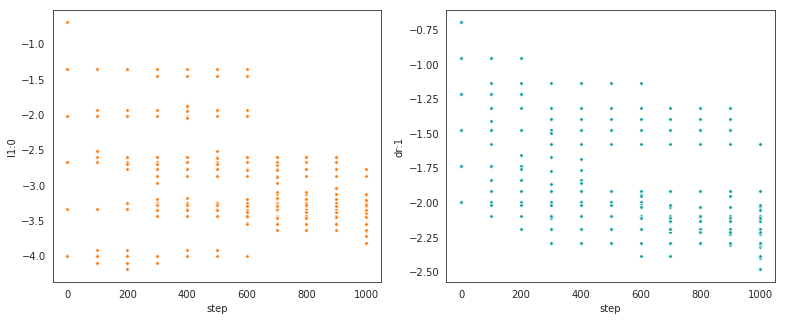
\includegraphics[width=\textwidth,height=\textheight,keepaspectratio]{hyperparameters_population2.png}
    \caption{l1 regularization (left) and dropout rate (right) values (in a log scale). Each marker represents the value for the corresponding hyperparameter of one worker at a specific step}
\end{figure}

Finally, if we observe both values at the same time (Fig. \ref{fig:evol2}), it very easy to see how the best hyperparameters now reside inside the grid. In the left figure, the points with pink colour (value 0 in the legend) represent the points of the original grid (right figure). Notice how this time some darker points (i.e., hyperparameters explored at a later stage during training) are inside the grid.

\begin{figure}[H]
    \label{fig:evol2}
    \centering
    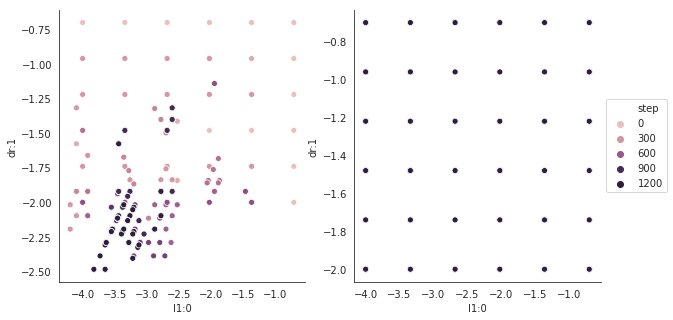
\includegraphics[width=\textwidth,height=\textheight,keepaspectratio]{hyperparameters_evolution2.png}
    \caption{l1 regularization value (x-axis, log scale) and dropout rate (y-axis, log scale) explored during PBT (left), and grid search (right). A darker colour represents a value explored in a later stage (step) during training.}
\end{figure}

\subsection{Convolutional Neural Network}
\label{sec:cnn}

For this experiment, we tune the original LeNet-5\cite{LeNet5} applied to handwritten character recognition using the MNIST dataset. The configuration of PBT is as follows.

\textbf{Hyperparameters}: we only allow to change the l1 regularization value and the dropout rate.

\textbf{Step}: each iteration does a step of gradient descent on a batch of data (32) using the Adam optimizer.

\textbf{Eval}: we evaluate a model computing the accuracy on the validation set.

\textbf{Ready}: a member is deemed ready to enter the exploit-explore phase every 300 iterations.

\textbf{Exploit}: same strategy previously explained.

\textbf{Explore}: we randomly perturb the hyperparameters by a factor of 0.2, 0.5, 1.5 or 2.

\subsubsection{Results}

\begin{figure}[H]
    \label{fig:training-curves3}
    \centering
    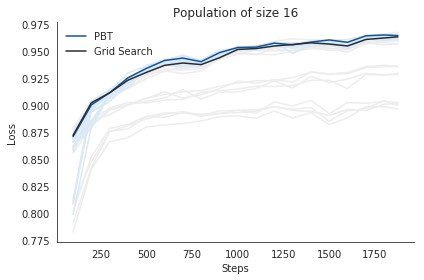
\includegraphics[scale=0.65]{training_curves3}
    \caption{Training curve for Grid Search and PBT (size 16). Y-axis represents accuracy (the higher, the better)}
\end{figure}

\begin{figure}[H]
    \label{fig:hyp3}
    \centering
    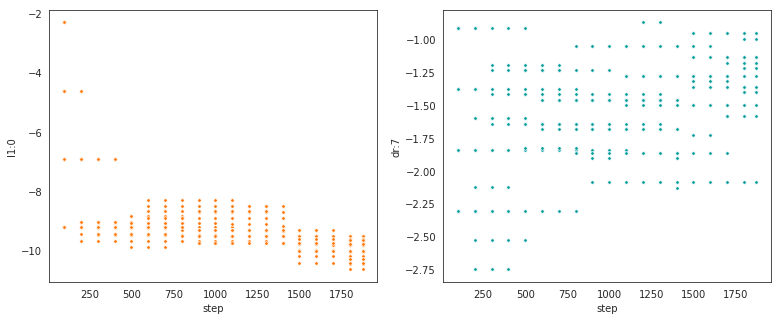
\includegraphics[width=\textwidth,height=\textheight,keepaspectratio]{hyperparameters_population3.png}
    \caption{l1 regularization (left) and dropout rate (right) values (in a log scale). Each marker represents the value for the corresponding hyperparameter of one worker at a specific step}
\end{figure}

\begin{figure}[H]
    \label{fig:evol3}
    \centering
    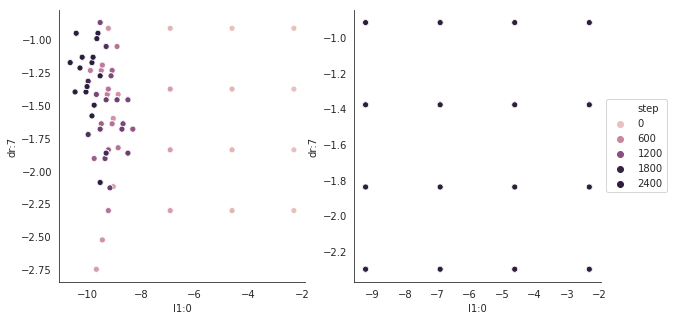
\includegraphics[width=\textwidth,height=\textheight,keepaspectratio]{hyperparameters_evolution3.png}
    \caption{l1 regularization value (x-axis, log scale) and dropout rate (y-axis, log scale) explored during PBT (left), and grid search (right). A darker colour represents a value explored in a later stage (step) during training.}
\end{figure}

Again, as in Sec. \ref{sec:goodgrid}, PBT beats Grid Search even when the best hyperparameters reside inside the grid. However, due to the lack of computational resources, we could not experiment with different population sizes.

\section{Conclusions, Discussion and Future Works}
\label{sec:discussion}

\subsection{Conclusions}

The qualitative results obtained show that PBT is consistently able to outperform grid search while training MLP and CNN models.

In particular, for the MLP model, the results reported in section \ref{sec:fcnn} show that in the case of an unfortunate choice of initial hyperparameters, PBT is able to identify optimal values outside the grid search space. This aspect should not be underestimated, as it is precisely demonstrating that this evolutionary approach can substitute a great deal of empirical decision making (i.e. the range of the hyperparameter grid). 

Regarding the amount of computational resources employed, PBT was able to beat the Grid search baseline with only one sixth of the total workers. Moreover, in case the hyperparameter grid contains already a set of good performing hyperparameters, PBT is able to obtain marginally better results.

As for the convolutional case, the results of section \ref{sec:cnn} suggests that PBT can obtain better results than grid search when the same resources are used.

\subsection{Discussion and Future Works}

Due to the budget at our disposal, both computationally-wise and time-wise, a set of decision has to be taken.

First of all, we decided to focus our investigation on a low dimensional hyperparameter space, as the computational cost associated will grow exponentially with the size of the grid. Due to this fact we decided to focus our comparison to grid search only, as it is considered to be marginally more proficient when the number of hyperparameters is low\cite{Bergstra:2012:RSH:2188385.2188395}. 
Future works should perform a comparison with random search rather than grid search and extend it to high dimensional problems.

Secondly, our results are only qualitative and lack the necessary statistical support that only a quantitative analysis can give. Concerning this aspects, we believe that the approach outlined by Bergstra in \cite{Bergstra:2012:RSH:2188385.2188395} should be followed to avoid any biased decision concerning the performance on the validation and test set (see section \ref{sec:literatureStudy} for further details).

Thirdly, one may argue that the sub-sampling of the grid explained in section \ref{sec:method} is rather subjective and could, by chance, favor PBT by giving especially good starting conditions and same results would not be achieved with a different choice of sub-sample. Future works following our method should perform different tries for a given population size, one per each possible sub-sampling of the hyperparameters grid, and treat the results accordingly\footnote{Considering the average and standard deviation when possible (large number of tries), or the min-max interval.}.

Finally, we were not able to estimate if PBT was able to outperform grid search with less computational resources while training CNNs. Future works should focus on this aspect.

We would also like to note that we didn't perform an in-depth analysis of the computational costs associated with the increased complexity of the PBT algorithm. As a matter of fact, PBT requires the weights of a successful individual to be copied into an under-performing one. From the wall-time perspective, this operation has a non-negligible cost often associated with the hardware at hand. 
Nevertheless, it is true that this complexity decreases by lowering the number of individuals and also that, given the faster convergence of PBT, the training process can be stopped earlier, thus saving even more time. This kind of trade-off should be the subject of a rigorous investigation.


\subsection{Sustainability and Ethics}

Machine learning applications are increasing the demand of computational resources used, which directly translates in an increase of power consumption. \textit{E-waste} is also an important aspect to consider, given that incrementally more performing computational hardware is being developed, thus rendering obsolete the older iterations. More proficient algorithms for hyperparameter tuning, as PBT seems to be, can only be seen as a technological improvement capable of reducing the power consumption and prolonging the life of older generation hardware. For this reason, we think that PBT is a positive contribution both from the ecocentric and anthropocentric standpoint.

The ethical aspects related to automatic hyperparameter tuning pertains to a more general family concerning the consequences of automation. Progress in the field can further reduce the need of understanding the dynamics of AI systems. Neural Networks are already models very hard to interpret. Using automatic hyperparameter optimization adds another layer of obscurity and, if it works well enough, there will be no push to investigate the inner dynamics of the hyperparameter optimization. In addition to this aspect, effective hyperparameter optimization will render the work of many data scientists useless. Although it is hard to tell if this will only be a liberation from a rather unappealing and annoying task that would set them free to invest their time more proficiently on other challenges.

\appendix
\section{Experimental Setup}

To carry out the experiments we developed PBT as explained in the original paper. However, in our implementation, all members are trained synchronously. The code is accessible at the following link:

\begin{itemize}
    \item \url{https://github.com/fdiazgon/pbt-keras}
\end{itemize}

Furthermore, given the lack of computational resources, we used Google Colaboratory for the experiment in Sec. \ref{sec:cnn} (CNN). The notebook can be accessed at the following link:

\begin{itemize}
    \item \url{https://drive.google.com/open?id=1hnVbX7ir_nHfehLRWFAoXhH1G-951Ygy}
\end{itemize}

For the rest of the experiments we used the following set-up:

\begin{itemize}
    \item Ubuntu 18.04.1 LTS
    \item Intel(R) Core(TM) i5-2410M CPU @ 2.30GHz
    \item 8GB RAM
    \item Tensorflow (CPU) v1.12.0
    \item Keras v2.2.4
\end{itemize}

\printbibliography
\end{document}


